%==============================================================================
% Sjabloon onderzoeksvoorstel bachproef
%==============================================================================
% Gebaseerd op document class `hogent-article'
% zie <https://github.com/HoGentTIN/latex-hogent-article>

% Voor een voorstel in het Engels: voeg de documentclass-optie [english] toe.
% Let op: kan enkel na toestemming van de bachelorproefcoördinator!
\documentclass{hogent-article}

% Invoegen bibliografiebestand
\addbibresource{}

% Informatie over de opleiding, het vak en soort opdracht
\studyprogramme{Professionele bachelor toegepaste informatica}
\course{Bachelorproef}
\assignmenttype{Onderzoeksvoorstel}
% Voor een voorstel in het Engels, haal de volgende 3 regels uit commentaar
% \studyprogramme{Bachelor of applied information technology}
% \course{Bachelor thesis}
% \assignmenttype{Research proposal}

\academicyear{2022-2023} % TODO: pas het academiejaar aan

% TODO: Werktitel
\title{Vul hier de voorgestelde titel van je onderzoek in}

% TODO: Studentnaam en emailadres invullen
\author{Ernsteeeer Aarden}
\email{ernst.aarden@student.hogent.be}

% TODO: Medestudent
% Gaat het om een bachelorproef in samenwerking met een student in een andere
% opleiding? Geef dan de naam en emailadres hier
% \author{Yasmine Alaoui (naam opleiding)}
% \email{yasmine.alaoui@student.hogent.be}

% TODO: Geef de co-promotor op
\supervisor[Co-promotor]{S. Beekman (Synalco, \href{mailto:sigrid.beekman@synalco.be}{sigrid.beekman@synalco.be})}

% Binnen welke specialisatierichting uit 3TI situeert dit onderzoek zich?
% Kies uit deze lijst:
%
% - Mobile \& Enterprise development
% - AI \& Data Engineering
% - Functional \& Business Analysis
% - System \& Network Administrator
% - Mainframe Expert
% - Als het onderzoek niet past binnen een van deze domeinen specifieer je deze
%   zelf
%
\specialisation{Mobile \& Enterprise development}
\keywords{Scheme, World Wide Web, $\lambda$-calculus}

\begin{document}

\begin{abstract}
  Hier schrijf je de samenvatting van je voorstel, als een doorlopende tekst van één paragraaf. Let op: dit is geen inleiding, maar een samenvattende tekst van heel je voorstel met inleiding (voorstelling, kaderen thema), probleemstelling en centrale onderzoeksvraag, onderzoeksdoelstelling (wat zie je als het concrete resultaat van je bachelorproef?), voorgestelde methodologie, verwachte resultaten en meerwaarde van dit onderzoek (wat heeft de doelgroep aan het resultaat?).
\end{abstract}

\tableofcontents

% De hoofdtekst van het voorstel zit in een apart bestand, zodat het makkelijk
% kan opgenomen worden in de bijlagen van de bachelorproef zelf.
%---------- Inleiding ----------------------------------------------------------

\section{Inleiding}%
\label{sec:inleiding}
Ransomware-aanvallen zijn één van de meest voorkomende aanvallen dat een organisatie kan treffen de dag van vandaag. Om gegevensverlies tegen te gaan in geval van een aanval moeten bedrijven altijd een back-upplan klaar hebben in geval van een incident. Het niet hebben van een back-upplan of het hebben van een suboptimaal plan kan leiden tot een groot verlies op financieel vlak. Daarnaast kan dit ook zorgen voor het verliezen van cruciale informatie en als laatste kan dit de reputatie van een organisatie sterk doen dalen, aangezien niemand in zee wilt gaan met een bedrijf dat niet goed beveiligd is of niet goed voorbereid is op uitzonderlijke incidenten. Om deze redenen is het van groot belang voor een bedrijf om een doordacht, robuust en veilig back-upplan te hebben.

Het doel van deze bachelorproef is het optimaliseren van het back-upplan van Forvis Mazars. Dit bedrijf maakt gebruik van 2 soorten databases in Azure, eenderzijds een PostgreSQL databank en anderzijds een MySQL databank. Van deze databanken worden er automatische alsook manuele back-ups gemaakt. De automatische back-ups gebeuren door Azure zelf en de manuele back-ups worden per database uitgevoerd. Stel dat applicatie A een nieuwe versie heeft, dan zal er eerst een back-up genomen worden van de database vooraleer de nieuwe versie uitgerold wordt. Echter zijn er nog bepaalde verbeteringen mogelijk, zoals het veiliger opslaan van deze back-ups met behulp van technieken als immutable storage en het instellen van geautomatiseerde dagelijkse, wekelijkse en maandelijkse back-ups. Daarbij is een belangrijk aandachtspunt dat de databanken beter beveiligd moeten worden tegen cyberaanvallen aangezien gegevens in zo'n situatie versleuteld of vernietigd kunnen worden.

De doelgroep van dit onderzoek bestaat uit de IT-professionals en vooral de systeembeheerders van Forvis Mazars, die verantwoordelijk zijn voor het beheer van de back-ups en de beveiliging van gegevens binnen de organisatie alsook het herstellen van alle gegevens na een incident.

De onderzoeksvraag die onderzocht zal worden is: ``Hoe kan de back-upstrategie van de Azure PostgreSQL en MySQL databases bij Forvis Mazars worden geoptimaliseerd door het implementeren van automatische back-ups en het veilig opslaan van deze back-ups om gegevensverlies te minimaliseren?'' In dit onderzoek wordt onderzocht hoe de bestaande back-upoplossingen kunnen worden verbeterd, zodat Forvis Mazars in geval van een incident goed voorbereid is en geen informatie verliest. De onderzoeksvraag kan onderverdeeld worden in volgende kleinere deelvragen:
\begin{itemize}
    \item Hoe veilig en betrouwbaar zijn de huidige back-upoplossingen van Forvis Mazars voor Azure PostgreSQL en MySQL databases?
    \item Welke rol speelt immutabele opslag in het beschermen van back-ups tegen ransomware en andere vormen van dataverlies?
    \item Wat zijn de belangrijkste uitdagingen bij het integreren van immutabele opslag met Azure cloud back-upsystemen?
    \item Hoe kan er voor de Azure PostgreSQL en MySQL databases een automatische back-upstrategie worden geïmplementeerd?
\end{itemize}

Het uiteindelijke doel van dit onderzoek is om ervoor te zorgen dat de Azure databanken van Forvis Mazars een geoptimaliseerd back-upplan hebben dat veilig en efficient is. Het plan moet immuun zijn tegen ransomware-aanvallen en daarnaast moet het ook geautomatiseerd zijn. Daarbij zal de tijd bij een herstel vanuit een back-up ook onderzocht worden. Om het back-upplan te testen zal er een Proof-of-Concept (PoC) opgesteld worden om alles grondig te testen in een testomgeving. 

%---------- Stand van zaken ---------------------------------------------------

\section{Literatuurstudie}%
\label{sec:literatuurstudie}
Bedrijven moeten hun data goed beschermen om succesvol te zijn. Echter vormen back-ups van de databases vaak een zwakke schakel in de beveiligingsketen van gegevensbescherming. Hoewel veel organisaties zich richten op het beveiligen van hun actieve databases, worden de back-ups vaak over het hoofd gezien, wat een groot risico met zich meebrengt. Back-ups worden meestal offsite opgeslagen, bijvoorbeeld op tape, en zijn daardoor vatbaar voor verlies of diefstal \autocite{Cherry2015}. Dit maakt het van essentieel belang om back-ups goed te beveiligen, bijvoorbeeld door encryptie. Echter, bij het kiezen van een encryptieoplossing is het belangrijk om een evenwicht te vinden tussen de sterkte van de encryptie en de impact op de prestaties van de server omdat sterke encryptie meer resources nodig heeft en het kan de beschikbaarheid van de back-ups veranderen. In de afgelopen jaren is er een scherpe toename van ransomware-aanvallen gericht op bedrijven, waarbij het aantal getroffen organisaties is gestegen van ruim 2.700 naar bijna 4.900 in slechts twaalf maanden. Deze toename laat zien hoe vastberaden en steeds slimmer ransomwaregroepen worden in hun aanvallen. Wat bijzonder zorgwekkend is voor de bedrijfswereld, is de trend van herhaalde aanvallen op bedrijven, waarbij sommige organisaties binnen korte tijd door meerdere ransomwaregroepen worden getroffen \autocite{Dikbiyik2024}. Dit wijst erop dat cybercriminelen actief profiteren van momenten van kwetsbaarheid om bedrijven in hun zwakste momenten opnieuw aan te vallen, wat de noodzaak voor robuuste preventieve maatregelen benadrukt.
\subsection{back-upstrategieën}%
\subsubsection{Full back-up}%
\begin{figure}[h] 
    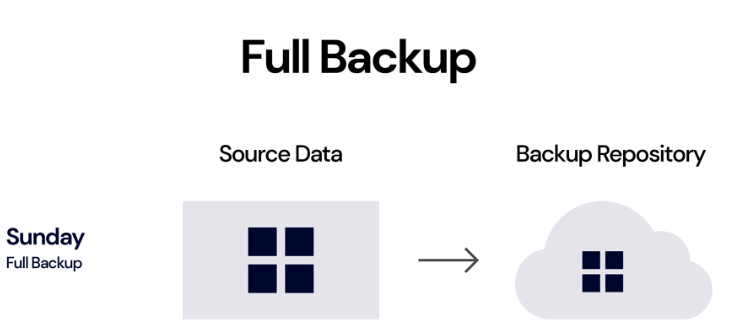
\includegraphics[width=0.5\textwidth]{img/fullb.png}  
    \caption{Representatie van een full back-up \autocite{Rivas2022}}   
    \label{fig:fullback-up}           
\end{figure}
Verschillende methoden en technologieën worden gebruikt om de veiligheid en betrouwbaarheid van data te garanderen. Een fundamentele back-upstrategie is de full back-up, waarbij de volledige inhoud van een bestandssysteem wordt gekopieerd naar een back-upapparaat \autocite{Beard2018}. Wanneer er zich een probleem voordoet, zoals het falen van een harde schijf, kan het hele bestandssysteem vanaf deze back-up volledig worden hersteld op een nieuwe schijf. Daarnaast kunnen ook individuele bestanden die verloren zijn gegaan, gemakkelijk worden teruggehaald uit de back-up. Dit soort back-up zorgt ervoor dat alle gegevens veilig zijn opgeslagen, maar heeft wel twee belangrijke nadelen. Ten eerste is het proces van het lezen en schrijven van het volledige bestandssysteem tijdsintensief, vooral bij grote hoeveelheden data. Ten tweede gebruikt het opslaan van een volledige kopie van het bestandssysteem veel opslagruimte, wat inefficiënt kan zijn wanneer de back-ups regelmatig worden gemaakt \autocite{Chervenak1998}.


\subsubsection{Incremental back-up}

Incremental back-ups zijn een efficiënte methode om alleen gewijzigde data sinds de laatste back-up op te slaan, wat tijd en opslag bespaart. In tegenstelling tot een volledige back-up, die alle data kopieert, richten incrementele back-ups zich enkel op nieuwe of aangepaste bestanden. Dit maakt ze sneller, maar hersteltijden kunnen langer zijn omdat meerdere incrementele back-ups nodig zijn naast de laatste volledige back-up. Recente onderzoeken hebben zich gericht op het optimaliseren van back-upstrategieën, met name voor databasesystemen. Zo zijn er modellen ontwikkeld die bepalen hoe vaak volledige en incrementele back-ups moeten worden uitgevoerd op basis van factoren zoals systeem-betrouwbaarheid, de hoeveelheid dataveranderingen en back-up-kosten \autocite{Zhao2024}. Er zijn ook varianten zoals differentiële back-ups, die alle veranderingen sinds de laatste volledige back-up bevatten, waardoor de hersteltijd korter kan zijn dan bij traditionele incrementele back-ups. Daarnaast zorgen moderne geautomatiseerde oplossingen voor continue incrementele back-ups, wat realtime herstelmogelijkheden biedt zonder noemenswaardige belasting van de productieomgeving \autocite{Qian2010}.
\begin{figure}[h] 
    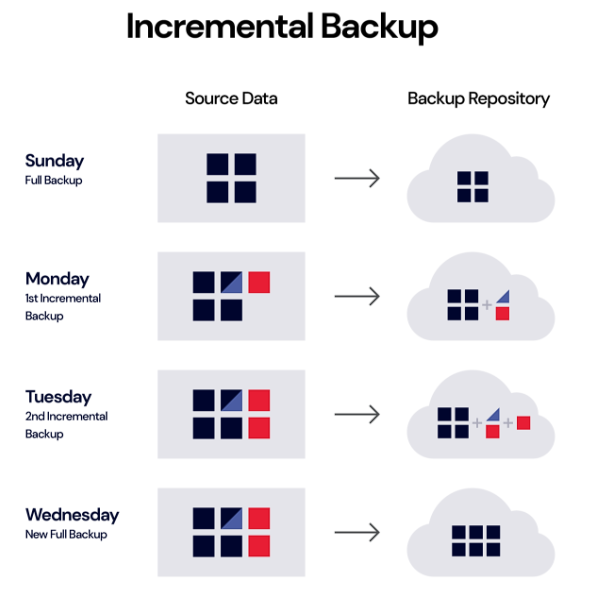
\includegraphics[width=0.5\textwidth]{img/incrementb.png}  
    \caption{Representatie van een incremental back-up \autocite{Rivas2022}}   
    \label{fig:incrback-up}           
\end{figure}


\subsubsection{Differentiële back-up}

Een differentiële back-up is een soort back-up waarbij alleen de data die sinds de laatste volledige back-up is veranderd of toegevoegd, wordt gekopieerd. In tegenstelling tot een incrementele back-up, die enkel de veranderingen sinds de laatste back-up opslaat, wordt er bij een differentiële back-up enkel de wijzigingen opgeslagen sinds de laatste full back-up . Dit komt doordat elke differentiële back-up alle wijzigingen sinds de meest recente volledige back-up bevat, waardoor de grootte van de back-up groter wordt naarmate er meer wijzigingen plaatsvinden. Een belangrijk voordeel van differentiële back-ups is de relatief snelle hersteltijd \autocite{Beard2018}. Om data te herstellen, is alleen de laatste volledige back-up en de meest recente differentiële back-up nodig, wat het herstelproces eenvoudiger en sneller maakt dan bij incrementele back-ups. Differentiële back-ups zijn bijzonder nuttig in omgevingen waar een snel herstelproces cruciaal is, zoals bij bedrijven die minimale downtime vereisen. Het nadeel van differentiële back-ups is dat de back-ups groter worden naargelang de tijd tussen de volledige back-ups. Elke nieuwe differentiële back-up bevat namelijk alle wijzigingen sinds de laatste volledige back-up, wat betekent dat deze geleidelijk groter wordt totdat er een nieuwe volledige back-up wordt gemaakt. Daarom is het belangrijk om een goede balans te vinden tussen de frequentie van volledige back-ups en differentiële back-ups.
 \begin{figure}[h]
     \centering
     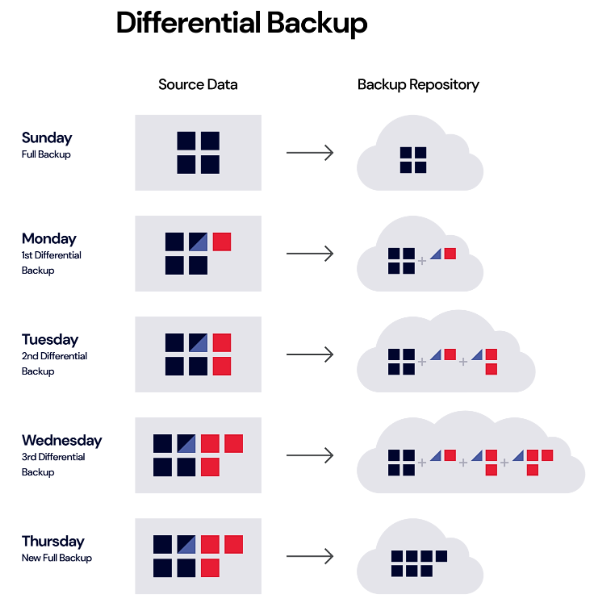
\includegraphics[width=0.5\textwidth]{img/diff.png}  
     \caption{Representatie van een differentiële back-up \autocite{Rivas2022}}   
     \label{fig:diffrback-up}           
 \end{figure}

\subsubsection{On-premise back-ups}
Bedrijven staan vaak voor de uitdaging om te beslissen of ze hun data on-premise opslaan of de voorkeur geven aan een cloud-service \autocite{Ali2024}. On-premise back-ups slaan gegevens lokaal op, meestal op fysieke schijven binnen het bedrijf zelf. Deze methode biedt bedrijven volledige controle over hun back-up- en gegevensbeheer. Een belangrijk voordeel van on-premise back-ups is dat data altijd beschikbaar is, zelfs zonder toegang tot het internet, wat nuttig is bij netwerkproblemen \autocite{Trovato2019}. Daarnaast hebben bedrijven volledige eigendom over de beveiliging van hun gegevens, aangezien de opslag lokaal blijft binnen het bedrijf. Hoewel deze methode geen terugkerende kosten aan externe providers met zich meebrengt, brengt het wel risico’s met zich mee, zoals schade door brand of overstromingen, en vraagt het om regelmatige onderhoud van de hardware. Het herstelproces is doorgaans sneller dan bij een cloudservice, wat van cruciaal belang kan zijn na een ransomware-aanval of een ander incident.
\subsubsection{Cloud-gebaseerde back-ups}
Cloud-gebaseerde back-ups zijn een populaire oplossing waarbij data extern wordt opgeslagen bij een bedrijf dat cloudservices aanbiedt. Dit biedt individuen en bedrijven de mogelijkheid om hun gegevens veilig op afstand te bewaren, zonder dat ze hoeven te investeren in fysieke opslagapparaten. Hoewel dit handig is om gegevensverlies te voorkomen bij hardware- of softwarestoringen, of onverwachte rampen, brengt het gebruik van cloud-opslag vaak aanzienlijke kosten met zich mee, vooral op de lange termijn \autocite{Obrutsky2016}. Naarmate je meer opslag nodig hebt is er altijd een mogelijkheid om te opschalen, dit is een groot voordeel van het gebruiken van een cloudservice. Echter, het waarborgen van de veiligheid van deze data is een cruciaal aandachtspunt, vooral omdat cloudproviders vaak niet open zijn over hoeveel kopieën van de data er zijn en waar deze precies worden opgeslagen. Om problemen zoals datalekken en foutieve verwijdering te voorkomen, zijn er nieuwe methoden zoals ``assured deletion'' ontwikkeld, waarmee klanten zeker weten dat hun gegevens permanent worden verwijderd op verzoek. Hierdoor kunnen bedrijven hun data met zekerheid beheren in de cloud terwijl gevoelige informatie veilig blijft \autocite{Rahumed2011}.


\subsubsection{Offline back-ups}
Offline back-ups zijn een traditionele methode waarbij data wordt opgeslagen op fysieke media, meestal externe harde schijven zonder tussenkomst van het internet. Het voornaamste voordeel is dat de data dan beveiligd is tegen online bedreigingen en er geen internettoegang nodig is om aan de data te geraken  \autocite{Edwards2022}. Een belangrijk voordeel is dat offline back-ups niet beïnvloed worden door stroomstoringen of internetuitval, waardoor ze een robuuste back-upoptie vormen voor gevoelige data. Echter, in tegenstelling tot on-premise back-ups, die vaak op dezelfde fysieke locatie als de IT-infrastructuur van een bedrijf worden opgeslagen, kunnen offline back-ups eenvoudig meegenomen en elders bewaard worden, waardoor ze extra bescherming bieden tegen fysieke rampen. Toch delen beide methoden het nadeel dat ze kwetsbaar zijn voor schade door ongelukken, diefstal of verlies, en moeten de fysieke apparaten op een veilige locatie opgeslagen worden \autocite{James2019}.

\subsubsection{Immutable storage}
Immutable storage is een type opslag waarbij data niet meer kan worden gewijzigd of aangepast vanaf het geback-upt is. Dit concept is cruciaal voor het waarborgen van de integriteit van belangrijke gegevens. Het idee achter immutability is dat bepaalde bestanden, nadat ze zijn gemaakt, niet meer mogen worden gewijzigd zonder de juiste autorisatie. Dit biedt een sterke bescherming tegen ongewenste wijzigingen en hierdoor kunnen hackers de gegevens niet aanpassen. Immutable storage speelt dus een belangrijke rol in het beschermen van systemen tegen cyberaanvallen. Bij aanvallen, waarbij hackers volledige toegang verkrijgen, kunnen onbeveiligde systemen worden gemanipuleerd of misbruikt. Immutable storage voorkomt dit, omdat de opgeslagen gegevens niet kunnen worden gewijzigd, zelfs niet door iemand met volledige toegang. Hierdoor wordt de integriteit van de data behouden en is het risico op schade door hackers aanzienlijk kleiner \autocite{Hasan2005}.

%---------- Methodologie ------------------------------------------------------
\section{Methodologie}%
\label{sec:methodologie}
In de eerste fase van het onderzoek zal er een grondige literatuurstudie worden uitgevoerd rond back-upstrategieën, ransomware-resistentie, en immutable storage met een overzicht van de state of the art van back-upstrategieën en immutabele opslag als deliverable. Wetenschappelijke papers, bedrijfscasussen en technische artikels zullen gebruikt worden om een theoretische basis aan te leggen en om de best-practices te achterhalen. Dit zal ook helpen om de onderzoeksvragen te beantwoorden. Daarnaast zal er een Proof-Of-Concept ontworpen worden waarbij onderzocht zal worden hoe er immutable back-ups gemaakt kunnen worden voor de back-ups van Forvis Mazars.  Daarnaast zal er een testomgeving opgezet worden om een ransomware-aanval na te bootsen en het systeem opnieuw op gang te krijgen. De deliverable voor de PoC is een werkende immutable back-upoplossing in Azure die tegen een ransomware-aanval bestendig is. Verder zal er een optimale back-upstrategie opgesteld worden met de state-of-the-art technieken. De literatuurstudie zal ongeveer 4 weken duren, de Proof-Of-Concept zal 4 weken duren en als laatst zal het rapport met de optimale verbeteringen 2 weken duren.

%---------- Verwachte resultaten ----------------------------------------------
\section{Verwacht resultaat, conclusie}%
\label{sec:verwachte_resultaten}
Het verwachte resultaat is dat door de implementatie van immutable storage en automatische back-ups, de back-upstrategie van Forvis Mazars zal worden verbeterd. Vooral de bescherming tegen ransomware en andere bedreigingen zal beter zijn door het gebruik van immutable storage, waarbij back-ups onveranderlijk worden opgeslagen en niet kunnen worden gemanipuleerd. Daarnaast zorgt de automatisering van de back-ups voor een efficiënter beheer, waarbij de manuele taken van het IT-team verminderd worden. Dit kan in de praktijk leiden tot meer consistente back-ups en een verbeterde betrouwbaarheid van het systeem. De resultaten zullen waarschijnlijk aantonen dat de combinatie van deze twee oplossingen zorgen voor een sterkere, efficiëntere en beter back-upstrategie.



\printbibliography[heading=bibintoc]

\end{document}